\documentclass[conference]{IEEEtran}

%\vfill\eject
% https://www.sharelatex.com/blog/2013/08/07/thesis-series-pt3.html

\usepackage{hyperref}
\usepackage{graphicx}
\usepackage{lscape}
\usepackage{tipa}
\usepackage{amsmath}
\usepackage{verbatim} % for \begin{comment}
\usepackage{caption} % for subfigures
\usepackage{subcaption} % for subfigures

\begin{document}
\title{CDN Improvements with Bloom Push and DHTs}

\author{
	\IEEEauthorblockN{Lisa Peters}
	\IEEEauthorblockA{\href{mailto:lisapeters.peters@gmail.com}{lisapeters.peters@gmail.com}}
	\and
	\IEEEauthorblockN{Nate Woods}
	\IEEEauthorblockA{\href{mailto:me@bign8.info}{me@bign8.info}}
}
\IEEEspecialpapernotice{Gianforte School of Computing at Montana State University}

\maketitle
\thispagestyle{plain}
\pagestyle{plain}

\section{Introduction}\label{sec:intro}
...

The rest of this paper is organized as follows.  We discuss background, related works, and technologies used in ~\ref{sec:back}.  Implementation details are in Section~\ref{sec:method}, followed an analysis of the system in Section~\ref{sec:results}..  Finally, we conclude in Section~\ref{sec:conclusion}. 

\section{Background}\label{sec:back}
\subsection*{Related Work}
\subsection*{Bloom Filters and DHT}
\subsection*{Chosen Technologies}
... ~\cite{docker} LEAVE AT LEAST ONE CITATION IN, OR LATEXT FREAKS OUT

\section{Method}\label{sec:method}
...

\begin{figure}[!h]
		\centering
		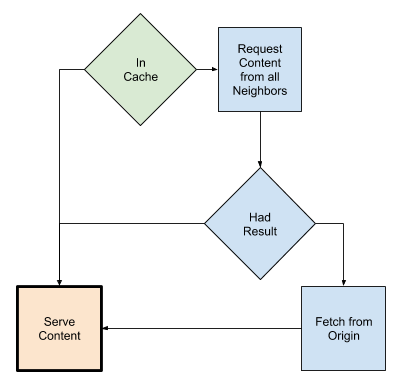
\includegraphics[width=0.49\columnwidth]{figures/cache_logic_before.png}
	\caption{Previous Implementation}
\end{figure}


\begin{figure}[!h]
	\centering
	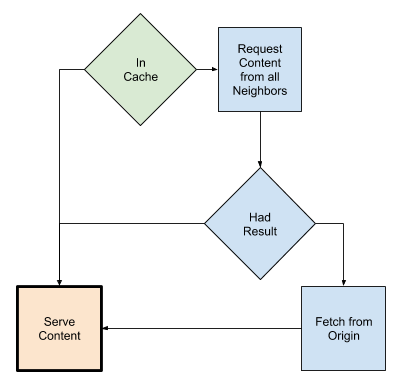
\includegraphics[width=0.49\columnwidth]{figures/cache_logic_before.png}
	\caption{DHT and Bloom Push Implementation}
\end{figure}

\section{Results}\label{sec:results}
...

\begin{figure}[!h]
	\centering
	\begin{subfigure}[b]{0.49\columnwidth}
		\centering
		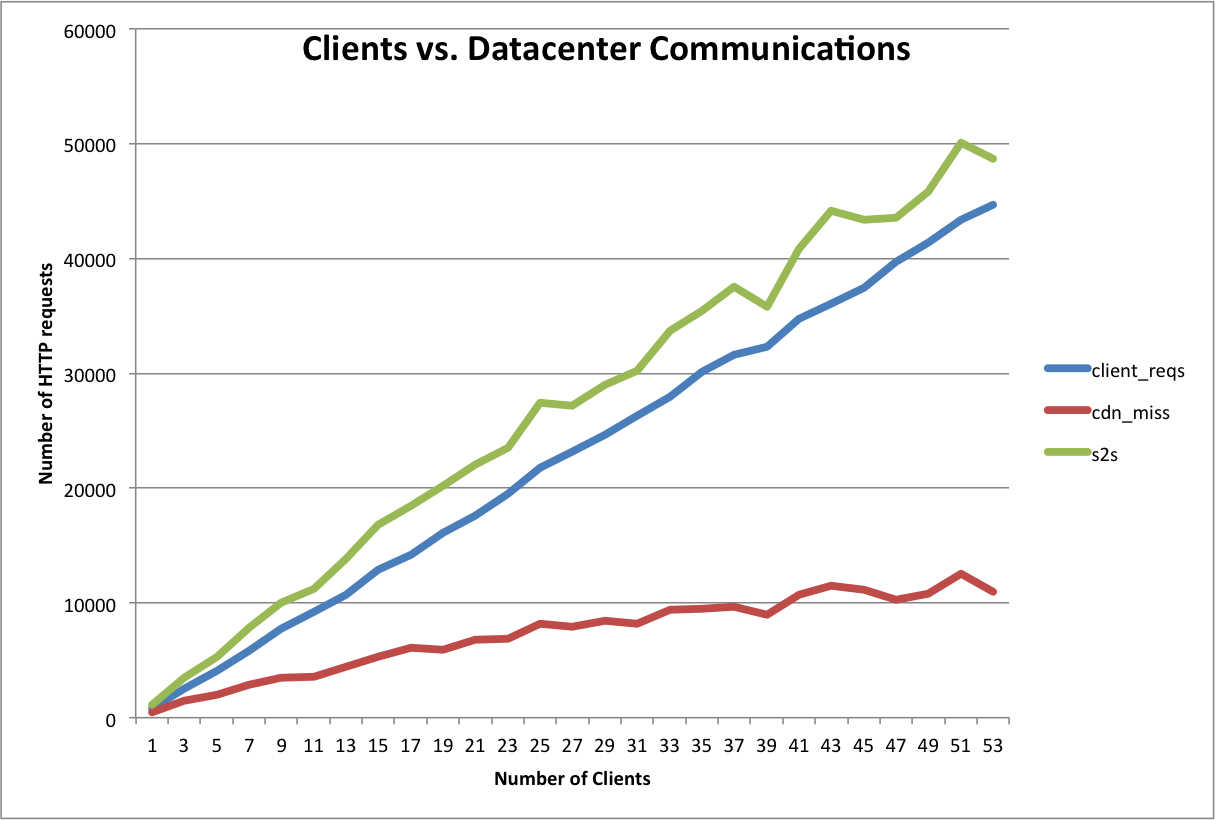
\includegraphics[width=\columnwidth]{figures/client-server.png}
	\end{subfigure}
	\begin{subfigure}[b]{0.49\columnwidth}
		\centering
		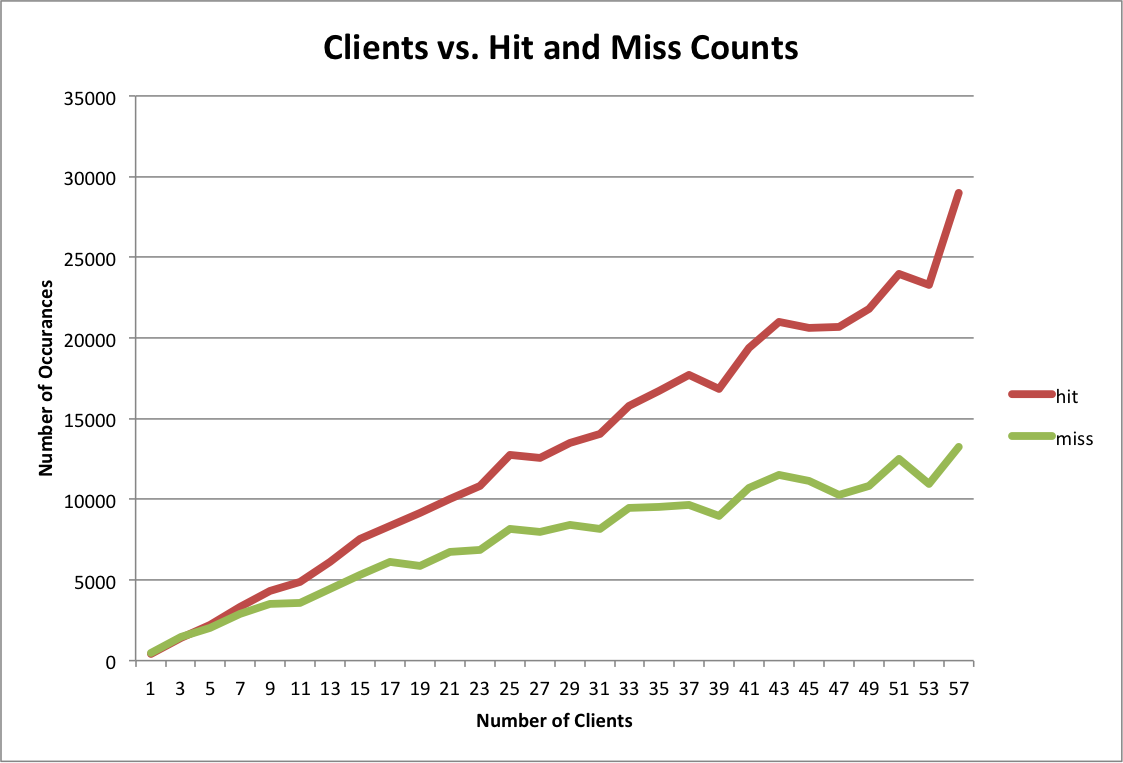
\includegraphics[width=\columnwidth]{figures/hit_miss_separate.png}
	\end{subfigure}
	\caption{Before}
\end{figure}

\begin{figure}[!h]
	\centering
	\begin{subfigure}[b]{0.49\columnwidth}
		\centering
		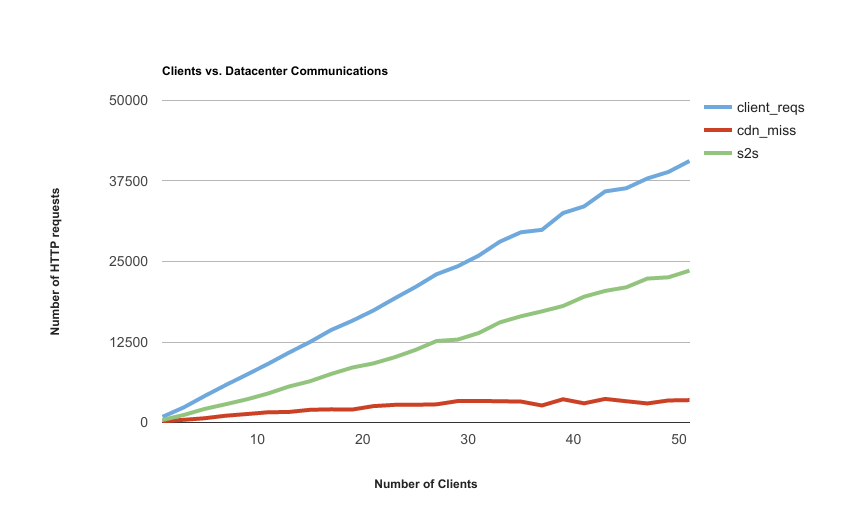
\includegraphics[width=\columnwidth]{figures/client-server_1.png}
	\end{subfigure}
	\begin{subfigure}[b]{0.49\columnwidth}
		\centering
		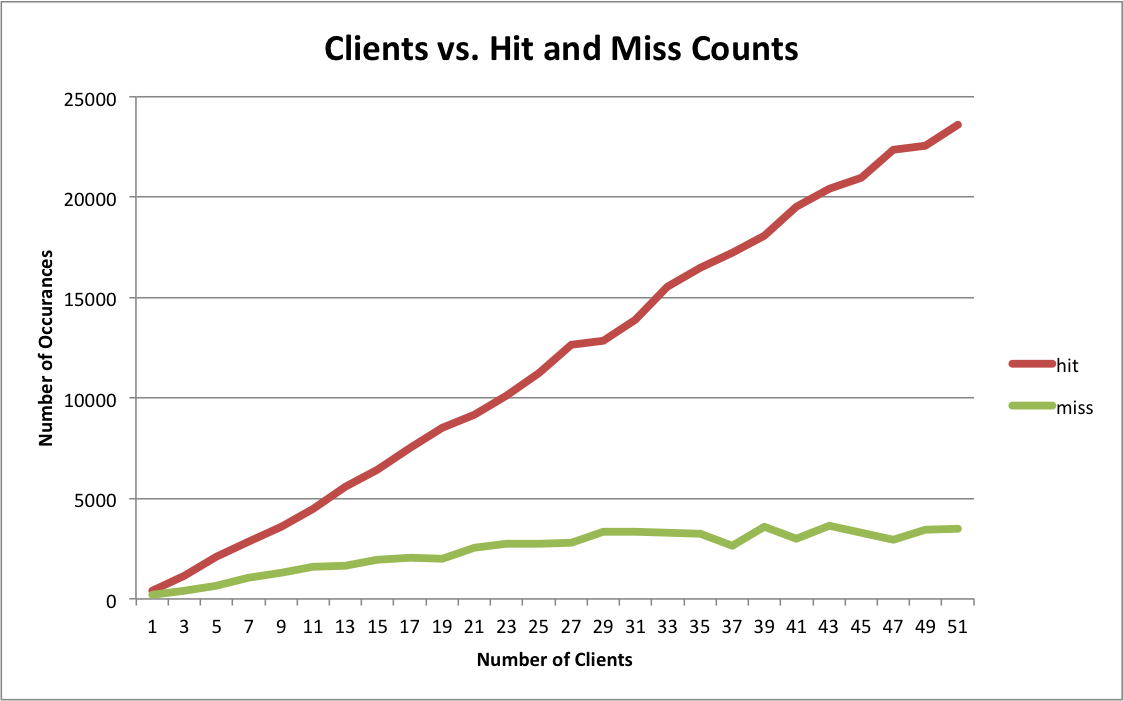
\includegraphics[width=\columnwidth]{figures/hit_miss_separate_1.png}
	\end{subfigure}
	\caption{After}
\end{figure}

\begin{figure}[!h]
	\centering
	\begin{subfigure}[b]{0.49\columnwidth}
		\centering
		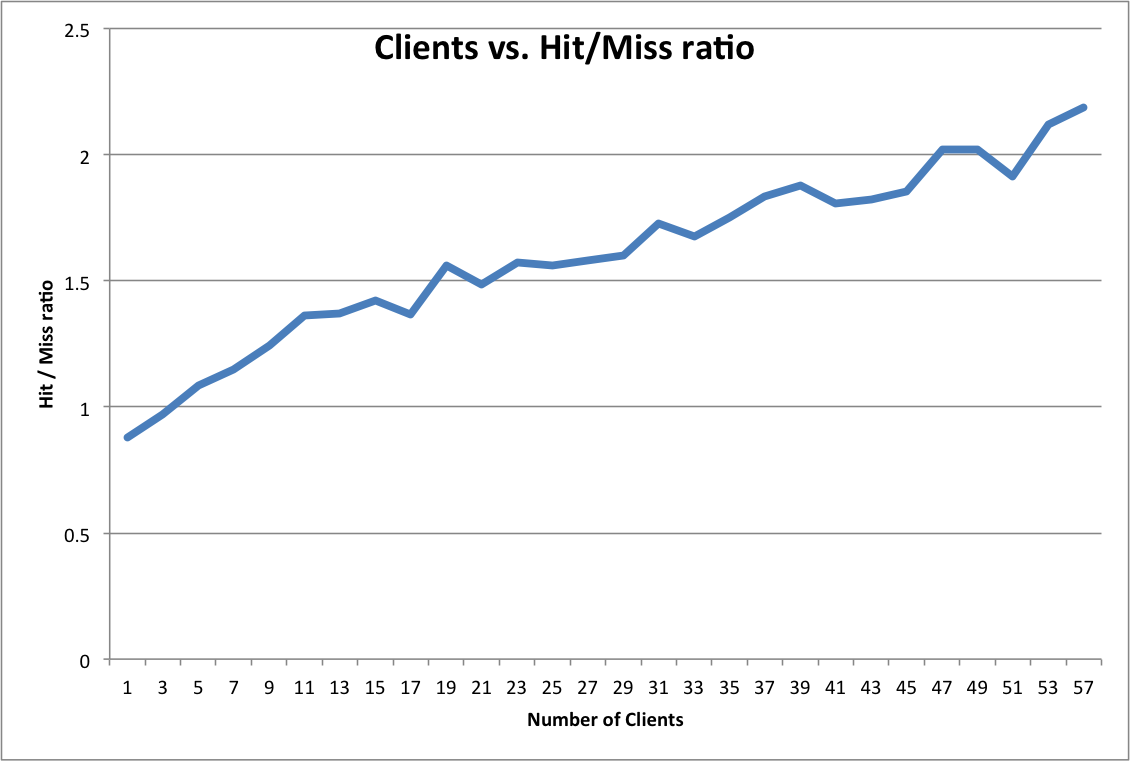
\includegraphics[width=\columnwidth]{figures/hit_miss.png}
	\end{subfigure}
	\begin{subfigure}[b]{0.49\columnwidth}
		\centering
		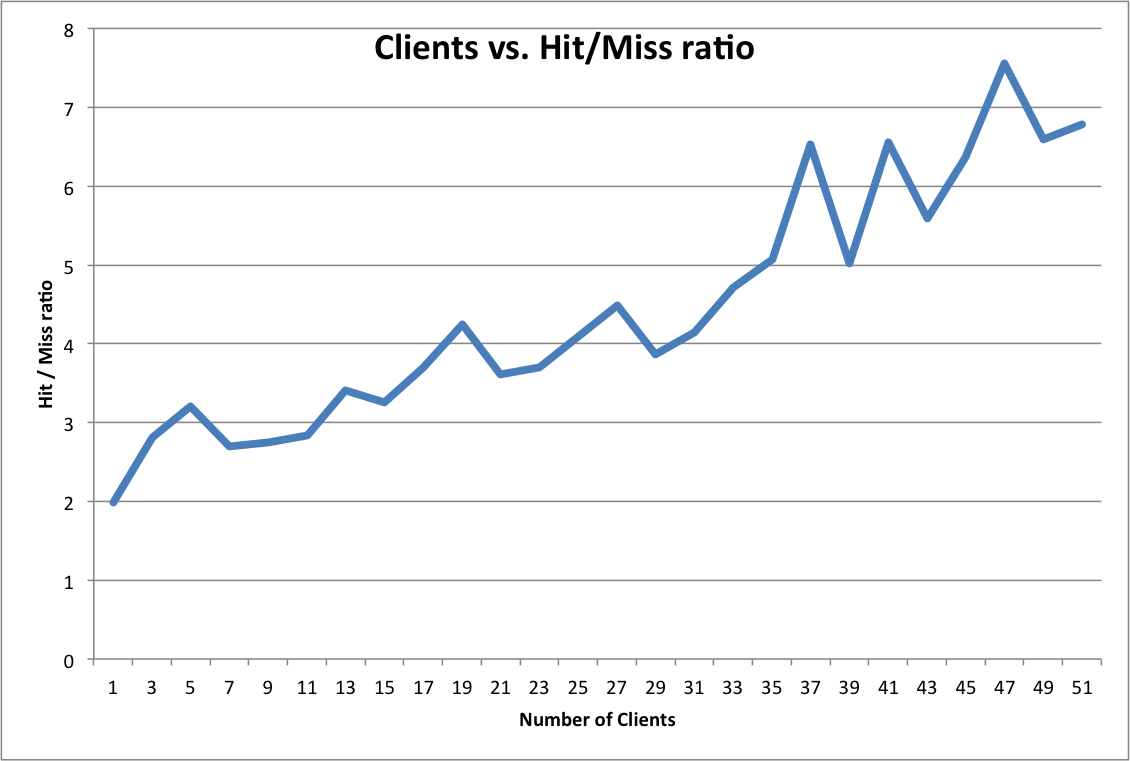
\includegraphics[width=\columnwidth]{figures/hit_miss_1.png}
	\end{subfigure}
	\caption{Hit/Miss Comparison}
\end{figure}

\begin{figure}[!h]
	\centering
	\begin{subfigure}[b]{0.49\columnwidth}
		\centering
		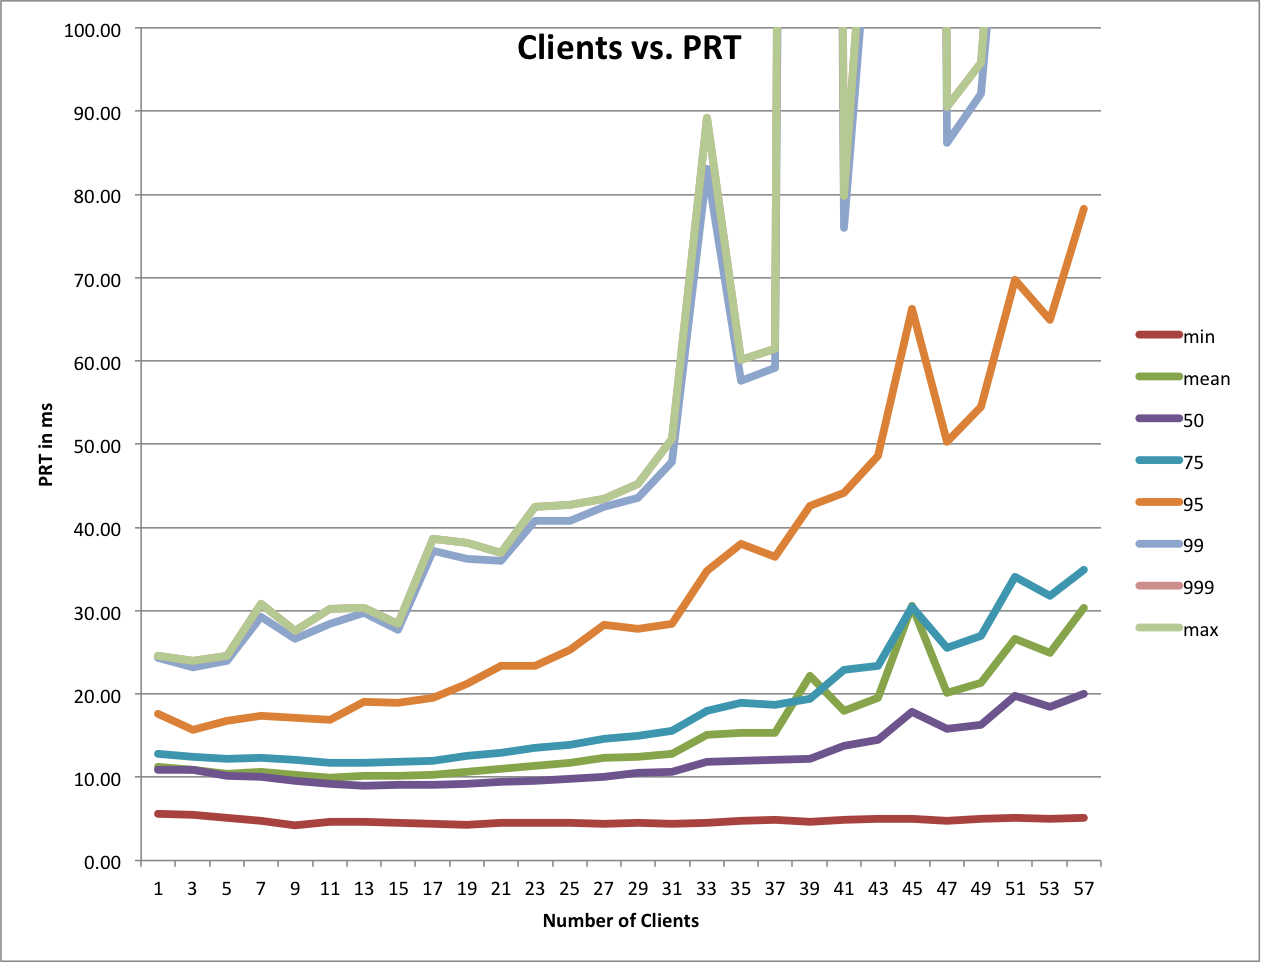
\includegraphics[width=\columnwidth]{figures/render.png}
	\end{subfigure}
	\begin{subfigure}[b]{0.49\columnwidth}
		\centering
		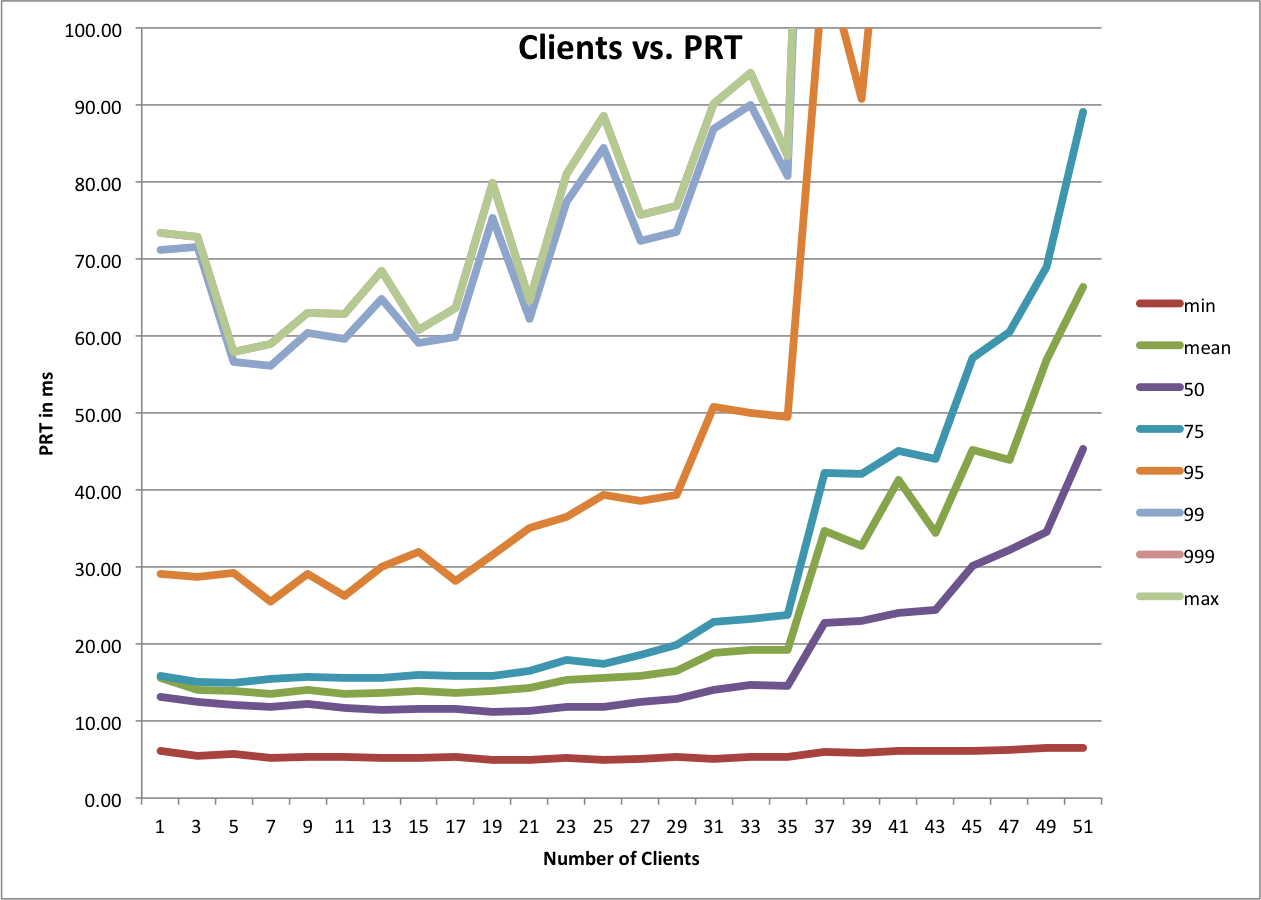
\includegraphics[width=\columnwidth]{figures/render_1.png}
	\end{subfigure}
	\caption{PLT Comparison}
\end{figure}


%In Figure~\ref{fig:abc} ...

%\begin{figure}[!h]
%	\centering
%	\begin{subfigure}[b]{0.49\columnwidth}
%		\centering
%		\includegraphics[width=\columnwidth]{img/abc.png}
%		\caption{abc}
%		\label{fig:abc}
%	\end{subfigure}
%	\begin{subfigure}[b]{0.49\columnwidth}
%		\centering
%		\includegraphics[width=\columnwidth]{img/sdf.png}
%		\caption{sdf}
%		\label{fig:sdf}
%	\end{subfigure}
%	\caption{abc + sdf}
%\end{figure}

...

\section{Conclusion}\label{sec:conclusion}
\subsection*{Future Work}

\bibliographystyle{plain}
\bibliography{cdn}

\end{document}
